% !TEX root = ../main.tex

% Summary section

\section{Conceptual summary}

The paper by \textcite{Mouli:2021} examines the problem of extrapolating patterns learned from training data from a single environment in a supervised setting to data from other environments. This problem context falls under the idea of \textit{domain adaptation} that has been explored in recent literature \parencite{Farahani:2020}. However, a key assumption in \citeauthor{Mouli:2021}'s work that distinguishes it from previous work in the literature is that the training data come from a single environment as opposed to multiple environments. Several previously proposed methods for domain adaptation---such as \textit{Invariant Risk Minimization} \parencite{Arjovsky:2020} (IRM)---rely on training data from multiple environments and therefore would fail under this problem context. \citeauthor{Mouli:2021} take a different approach by viewing extrapolation as counterfactual reasoning in a specified structural causal model (SCM) and assuming known (linear automorphism) group structures on the non-causal mechanisms. Under this formulation, \citeauthor{Mouli:2021} introduce a learning framework for the single-environment context that is able to learn invariances that do not contradict the data. In this conceptual summary, we review the key contributions of the paper by \textcite{Mouli:2021} and discuss the strengths and weaknesses of their approach.


\subsection{Key differences from previous work}

Various methods for domain adaptation have been proposed in the literature, and how the work by \textcite{Mouli:2021} relates to these methods are highlighted in their paper. For example, methods based on causal inference such as IRM and \textit{Independent Causal Mechanisms} \parencite{Parascandolo:2018} (ICM) broadly involve learning some internal representation of the data that is invariant to environment non-causal mechanisms. The invariant representation is learned from the training data which come from multiple environments. When the data come from a single environment, the representation cannot determine which aspects of the data are environment-specific and so the representation is unlikely to extrapolate to new environments. The learning framework proposed by \citeauthor{Mouli:2021} works with single-environment data and has an advantage over existing methods in these settings.
\\

Another well-known approach to domain adaptation is based on data augmentation \parencite{Chen:2020} where training is done with not only the original data but also proper transformations of the data. \citeauthor{Mouli:2021} explains that data augmentation is a type of \textit{forced group invariance} (i.e., forced \textit{G-invariance}) where certain transformations of the data may actually introduce contradictions (e.g., trying to enforce rotation invariance in images of digits, but digits 6 and 9 are not invariant to 180$^o$ rotations). \citeauthor{Mouli:2021}'s proposed learning framework aims to learn only the invariances that do not contradict the training data.


\subsection{Main contributions}

The main contributions of the paper by \textcite{Mouli:2021} include a formulation of the single-environment extrapolation problem, a learning framework based on the formulation that aims to learn the non-contradicting invariances, and an empirical evaluation of standard neural networks versus neural networks trained using the proposed learning framework.
\\

\citeauthor{Mouli:2021}'s formulation of the single-environment extrapolation problem is based on the ICM literature where a SCM is used to describe the input variables that influence or are irrelevant to the internal representation across environments (\todo cite?). Extrapolation is then seen as counterfactual reasoning where being able to extrapolate to different environments is tied to the representation being invariant to interventions on non-causal environment variables. \citeauthor{Mouli:2021} extends this idea by assuming known linear automorphism groups acting on the non-causal variables, in which case extrapolation of a representation is equivalent to the representation being counterfactually invariant to a group (i.e., \textit{CG-invariant}). This extension is the crux of the formulation that allows the proposed learning framework to work with single-environment data.
\\

The learning framework proposed by \citeauthor{Mouli:2021} aims to learn an internal representation that is CG-invariant to specified groups that do not contradict the training data. \citeauthor{Mouli:2021} show that CG-invariance is stronger than G-invariance (Theorem 1), but when the group acting on the non-causal variables is a normal subgroup of the group acting on all variables, then G-invariance also implies CG-invariance (Theorem 2). These results establish the group conditions under which it is sufficient for the model to learn G-invariances in place of CG-invariances.
\\

The challenge in learning the G-invariances that do not contradict the training data is due to the fact that the set of non-causal variables among all variables is unknown. To learn the invariances for the unknown set, \citeauthor{Mouli:2021} require the groups to be (finite) linear automorphisms. A group-invariant transformation can be constructed by averaging over members of the group (the \textit{Reynolds operator}, Lemma 1). For linear transformations, the averaged transformation is a projection operator with eigenvalues 1 and 0. The left eigenspace spanned by eigenvectors with eigenvalue 1 represents the space of transformations that are invariant to the group (Lemma 2). \citeauthor{Mouli:2021} exploit this property by computing the intersection of these subspaces for all subsets of the set of groups, and the set of invariant subspaces can then be partially ordered by the size of their corresponding subset (i.e., the \textit{strength} of the invariance, Theorem 3). The objective optimized in the learning framework then includes a regularization term that encourages learning a representation with the strongest G-invariance that does not significantly contradict the data. The key aspects of this learning framework include needing to specify known groups, requiring the groups to be linear automorphisms and, in doing so, being able to automatically learn the G-invariances that do not (significantly) contradict the data.
\\

\citeauthor{Mouli:2021} evaluated neural networks trained using their proposed learning framework on various image tasks and array tasks. Their results broadly suggest that
\begin{enumerate}

\item
standard neural networks do well when interpolating but not when extrapolating,

\item
neural networks trained with forced G-invariances do poorly when interpolating but do well when extrapolating, and

\item
neural networks trained with their learning framework generally do well when interpolating and when extrapolating.

\end{enumerate}

 
\subsection{Limitations}

The main limitations of the learning framework proposed by \textcite{Mouli:2021} originate from the assumptions made. To allow for single-environment data, the framework requires that the invariance groups acting on the data are known and specified. Furthermore, to enable automatic learning of invariances that do not contradict the training data, the groups are also restricted to be linear automorphisms. This framework cannot be used if no linear group structure could placed on the transformations that act on the data.
\\

These limitations naturally point to directions for future work where non-linear groups or even non-groups of transformations are considered. It is also worth investigating if a method for single-environment extrapolation that does not require known groups is possible.


\newpage


\section{Technical summary}

The technical components of the paper by \textcite{Mouli:2021} include the proposed learning framework and the theoretical results that justify its usage in the given setting. In this technical summary, we introduce the formulation and notation of the single-environment extrapolation problem, discuss the assumptions made in the formulation, and describe the proposed learning framework for use under the formulated setting.


\subsection{Single-environment extrapolation setting}

In the context of single-environment extrapolation described by \textcite{Mouli:2021}, the goal is to learn (in a supervised learning setup) a prediction model where the output  only depends on information that is relevant across different environments. The challenge is learning which information is relevant given only training data from a single environment. To simplfy this problem, \citeauthor{Mouli:2021} assume a known set of groups $\calG_1,\ldots,\calG_m$ of linear transformations acting on the data, and the objective is to learn an internal representation of the data that is invariant to an unknown subset of groups assumed to be irrelevant to the output. \citeauthor{Mouli:2021} works under an ICM setup where the SCM in Figure~\ref{fig:scm} is assumed.

\begin{figure}[H]
\centering
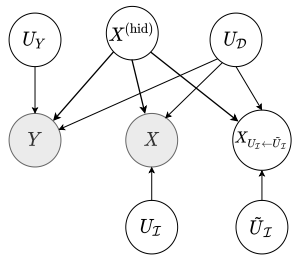
\includegraphics[width=0.4\textwidth]{scm.png}
\caption{Structural causal model assumed in single-environment extrapolation. Grey nodes are observed variables. Figure taken directly from \parencite{Mouli:2021}.}
\label{fig:scm}
\end{figure}

The variables in the assumed SCM are defined as follows:
\begin{itemize}

\item
$\calD$, $\calI$: (unknown) disjoint sets of indices that describe the groups of transformations that are relevant and irrelevant to the output, respectively. $\calD\cup\calI=\{1,\ldots,m\}$.

\item
$U_Y$, $U_\calI$, $U_\calD$, $\tildeU_\calI$: independent latent variables that influence the value of the variable(s) that they point to.

\item
$X^{\text{(hid)}}$: some unknown canonical form of the observed input $X$.  It is assumed that given $U_\calD$ and $U_\calI$, $X$ was obtained from an ordered sequence of transformations on the canonical form, i.e.,
\[
X=T_{U_\calD,U_\calI}\circ X^{\text{(hid)}}
\]
where transformations
\[
T_{U_\calD,U_\calI}=T_\calI^{(1)}\circ T_\calD^{(1)}\circ T_\calI^{(2)}\circ\ldots
\]
make up the overgroup $\calG_{\calD\cup\calI}$, $T_\calD^{(j)}$ is a transformation in group $\calG_j$ from the overgroup $\calG_\calD=\langle\cup_{j\in\calD}\calG_j\rangle$, and $T_\calI^{(i)}\in\calG_i\subset\calG_\calI=\langle\cup_{i\in\calI}\calG_i\rangle$. Note that $\calG_\calI$ is also assumed to be a normal subgroup of $\calG_{\calD\cup\calI}$.

\item
$Y$: observed output assumed to be generated by
\[
Y = h(X^{\text{(hid)}},U_\calD,U_Y)
\]
where $h$ is a deterministic function.

\item
$X_{U_\calI\leftarrow\tildeU_\calI}$: counterfactual variable to $X$ where $U_\calI$ has been replaced by $\tildeU_\calI$, i.e.,
\[
X_{U_\calI\leftarrow\tildeU_\calI} = T_{U_\calD,\tildeU_\calI}\circ X^{\text{(hid)}} \;.
\]

\end{itemize}

Given the SCM, the goal is to learn a representation $\Gamma:\calX\rightarrow\bbR^d$, $d\geq 1$, that is CG-invariant, i.e.,
\[
\Gamma(X) = \Gamma(X_{U_\calI\leftarrow\tildeU_\calI})
\]
where the equality implies $\Gamma(X_{U_\calI\leftarrow u})=\Gamma(X_{U_\calI\leftarrow u'})$ for all $u\in\supp(U_\calI)$, $u'\in\supp(\tildeU_\calI)$. The representation $\Gamma$ is fed into a learned link function $g:\bbR^d\rightarrow \text{Im} P(Y=y|X)$, $\text{Im} P(\cdot)$ being the image of $P(\cdot)$, which produces the prediction of the model, i.e.,
\[
\hat{Y}|X \sim g(\Gamma(X)) \;.
\]
For training data $X^\text{(tr)}$, if
\[
Y|X^\text{(tr)} \equdist \hat{Y}|X^\text{(tr)}\sim g_{\text{true}}(\Gamma_{\text{true}}(X^\text{(tr)}))
\]
and $\Gamma_\text{true}(X) = \Gamma_\text{true}(X_{U_\calI\leftarrow\tildeU_\calI})$, then $g_\text{true}\circ\Gamma_\text{true}$ extrapolates to test data $X^\text{(te)}$ in the sense that
\[
Y|X^\text{(te)} \equdist \hat{Y}|X^\text{(te)}\sim g_{\text{true}}(\Gamma_{\text{true}}(X^\text{(te)})) \;.
\]


\subsection{Assumptions in single-environment extrapolation}

\textcite{Mouli:2021} make a number of assumptions in the setup described in the previous section in order to simplify the extrapolation problem and to allow for a feasible learning framework. Compared to previous work in the literature, the main assumptions that are unconventional involve the transformation groups acting on the data.
\\

Unlike previous work that assumes the availability of training data from multiple environments, the problem context considered by \citeauthor{Mouli:2021} specifically considers data from a single environment. Without additional information that suggests how data from different environments may differ, it is likely impossible to learn what pieces of information are environment-specific and irrelevant to the output. \citeauthor{Mouli:2021} get around this issue by assuming a priori knowledge of how environments may differ in the form of transformation groups. The given groups specify the potential ways data from different environments may differ, and it is left to the learning framework to ``unlearn'' the given groups that contradict the training data.
\\

Furthermore, \citeauthor{Mouli:2021} assume that the subset $\calG_\calI$ of groups is a normal subgroup of the overgroup $\calG_{\calD\cup\calI}$. This assumption is a consequence of Theorems 1 and 2, which together state that CG-invariances are G-invariances, but G-invariances are CG-invariances only when $\calG_\calI\unlhd\calG_{\calD\cup\calI}$. \todo


\subsection{Learning framework for single-environment extrapolation}

\todo Under the setting described in the previous section, \textcite{Mouli:2021} propose a framework for learning the CG-invariant representation.